\documentclass[12pt]{article}

\usepackage{amsmath, amssymb, amsthm}
\usepackage{enumerate}
\usepackage{changepage}
\usepackage{pgfplots, pgfplotstable}

\title{CS325 Winter 2013: Implementation 1}
\author{
    Daniel Reichert \\
    Trevor Bramwell
}
\date{\today}

\begin{document}
\maketitle

\section*{Asymptotic Analysis}
    \begin{enumerate}

    \item In algorithm 1 the problem is not branched into any subproblems.
          With the nested for loops there is a comparison made between
          every element in the input, leading to an intuitive asymptotic
          complexity of $O(n^2)$

	\item In algorithm 2 the problem is branched into $2$ subproblems
          for size $n/2$ at each level.  It is similar to algorithm 3, but the
		  counting of inversions is done inefficiently.  This is represented in
		  the master theorem as the cost of combining the subproblems.  Because of the
		  naive nature of the merge and count approach, the additional cost of combining
		  ends of being the dominating term in the master theorem as it is greater than
		  $n log n$.  Every time that two lists are merged, each element is compared to
		  every other element.  Since there are $log_2 n$ merges that take place and
		  each merge compares itself to every other item in the list this is a $O(n^2 log n)$ algorithm.

    \item In algorithm 3 the problem is branched into $2$ subproblems of size
          $n/2$ at each level.  The depth of the problem is $log_2 n$
          and the width is $n^{log_2 2}$.  From the master theorem we know
          that $A/B^D$ determines the run time complexity.  Since this
          case is $2/2^1 = 1$, we know that the Asymptotic complexity is
          $O(n log n)$.

    \end{enumerate}

\section*{Testing}

\begin{center}
\begin{tabular}{|c|c|}
\hline
verify.txt & test\_input.txt \\ \hline
9670  & 249310 \\ \hline
10567 & 252709 \\ \hline 
9282  & 253719 \\ \hline 
9269  & 249315 \\ \hline 
9675  & 247789 \\ \hline 
10378 & 254833 \\ \hline 
9911  & 239844 \\ \hline 
9790  & 257527 \\ \hline 
9580  & 241669 \\ \hline 
9965  & 255628 \\
\hline
\end{tabular}
\end{center}

\section*{Extrapolation and Interpretation}

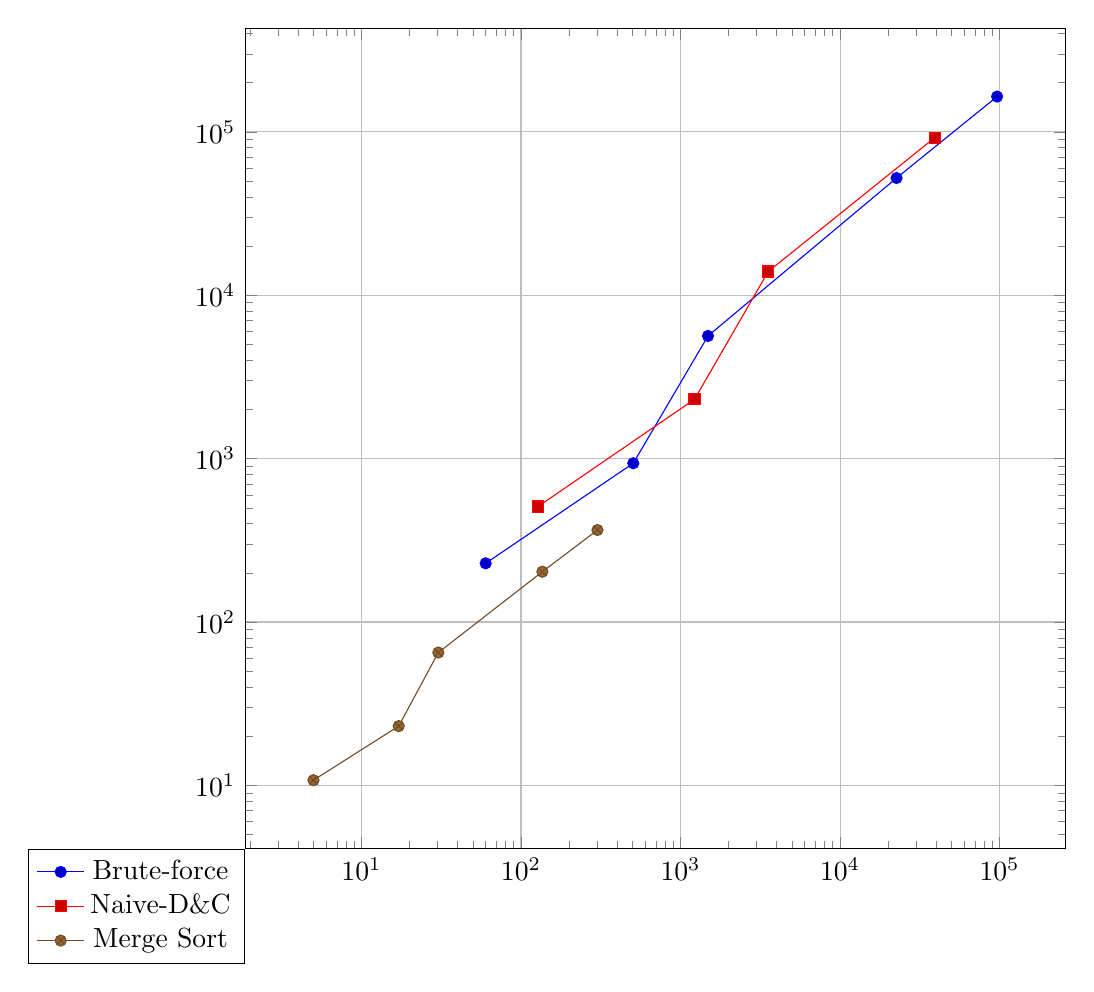
\begin{tikzpicture}
    \begin{loglogaxis} [
        legend style={at={(0,0)}, anchor=north east},
        grid=major,
        height=12cm,
        width=12cm,
    ]
    %\addplot coordinates {
    %    (57.154179, 224.262953)
    %    (488.316059, 897.155046)
    %    (1450.166941, 5447.463036)
    %    (21649.191856, 49863.325834)
    %    (91092.915058, 153462.900877)};

    \addplot coordinates {
        (60.023069, 228.663921)
        (505.338907, 936.666012)
        (1486.296177, 5632.760048)
        (22593.914032, 52147.319078)
        (96452.900171, 164262.082100)};
    \addlegendentry{Brute-force}

    \addplot coordinates {
        (127.677917, 508.983135)
        (1223.464966, 2305.993080)
        (3546.563864, 13964.954853)
        (39254.812002, 92156.149149)};
    \addlegendentry{Naive-D\&C}

    \addplot coordinates {
         (4.997969, 10.764122)
         (17.102003, 23.066998)
         (30.307055, 65.042973)
         (136.113167, 203.222990)
         (301.517010, 365.700006)};
    \addlegendentry{Merge Sort}

    \end{loglogaxis}
\end{tikzpicture}

\end{document}
